% =====================================================================
%  Elastic LLM Inference Gateway - Final Report
%  CS363 Cloud Computing, Department of CSE, NITK Surathkal
%
%  Compile with pdfLaTeX (Overleaf default), twice for references:
%      pdflatex report.tex && pdflatex report.tex
%  Figures are looked up in figures/ (Overleaf upload) and ../plots/ (repository).
%  Same content as report/report.md; every number comes from report/evidence/.
% =====================================================================
\documentclass[11pt,a4paper]{article}

% ---- fill in if you want the instructor on the title page (leave empty to omit) ----
\newcommand*{\instructor}{}

\usepackage[T1]{fontenc}
\usepackage[utf8]{inputenc}
\usepackage{lmodern}
\usepackage[a4paper,margin=2.3cm]{geometry}
\usepackage{microtype}
% keep "--cpus" as two hyphens in typewriter text (no en-dash ligature)
\DisableLigatures[-]{encoding = T1, family = tt*}
\usepackage{flafter}   % a float never appears before the text that introduces it
\usepackage{amsmath}
\usepackage{graphicx}
\usepackage{booktabs}
\usepackage{array}
\usepackage{tabularx}
\usepackage{enumitem}
\usepackage[font=small,labelfont=bf]{caption}
\usepackage{xcolor}
\usepackage{listings}
\usepackage{tikz}
\usetikzlibrary{arrows.meta,positioning,fit,backgrounds}
\usepackage[hidelinks]{hyperref}

\graphicspath{{figures/}{../plots/}}
% bullet lists stay in one piece and stay with the sentence that introduces them
\setlist{itemsep=2pt,topsep=4pt,beginpenalty=10000,midpenalty=10000}
\setlength{\parskip}{4pt}
\renewcommand{\arraystretch}{1.2}
\setlength{\emergencystretch}{2em}   % long file names: stretch a line rather than overflow
\setcounter{tocdepth}{2}
% keep every block in one piece: a paragraph never breaks across pages (it moves whole to the
% next page) and pages may end short instead of being stretched
\interlinepenalty=10000
\clubpenalty=10000
\widowpenalty=10000
\raggedbottom
\definecolor{titleblue}{RGB}{22,52,112}
\renewcommand{\topfraction}{0.9}
\renewcommand{\textfraction}{0.1}
\renewcommand{\floatpagefraction}{0.8}
\makeatletter                        % float-only pages: floats at the top, not spread out
\setlength{\@fptop}{0pt}
\setlength{\@fpsep}{14pt plus 1fil}
\setlength{\@fpbot}{0pt plus 1fil}
\makeatother
\newcolumntype{L}{>{\raggedright\arraybackslash}X}
\newcolumntype{P}[1]{>{\raggedright\arraybackslash}p{#1}}

% identifiers, file names and config keys (underscores are safe inside)
\DeclareRobustCommand{\code}[1]{\texttt{\detokenize{#1}}}
\newcommand{\rng}[2]{[#1--#2]}

\lstset{basicstyle=\ttfamily\footnotesize, breaklines=true, columns=fullflexible,
        frame=single, rulecolor=\color{black!30}, backgroundcolor=\color{black!3},
        xleftmargin=4pt, xrightmargin=4pt, aboveskip=6pt, belowskip=6pt}

\hypersetup{pdftitle={Elastic LLM Inference Gateway - Final Report},
            pdfauthor={B Darshan Sai Naath, Parmeet Singh Saini, Vishal Murugan, Jiya Jayaprakash}}

\begin{document}

% =====================================================================
\begin{titlepage}
% page border: a single frame
\begin{tikzpicture}[remember picture, overlay]
  \draw[titleblue, line width=1.5pt]
    ([xshift=1.2cm, yshift=-1.2cm]current page.north west) rectangle
    ([xshift=-1.2cm, yshift=1.2cm]current page.south east);
\end{tikzpicture}
\centering
\vspace*{0.4cm}
{\Large\bfseries\color{titleblue} National Institute of Technology Karnataka, Surathkal\par}
% optional: put the institute logo at figures/nitk_logo.png and it appears here
\IfFileExists{figures/nitk_logo.png}{\vspace{14pt}\includegraphics[height=3cm]{nitk_logo.png}\par}{}
\vspace{14pt}
{\Large Department of Computer Science and Engineering\par}
\vfill
{\Large\bfseries Cloud Computing (CS363) -- Course Project\par}
\vspace{1cm}
{\color{titleblue}\rule{\textwidth}{1.4pt}}\par\vspace{16pt}
{\fontsize{34}{42}\selectfont\bfseries Elastic LLM\\[2pt] Inference Gateway\par}
\vspace{14pt}
{\Large\itshape Scheduling, routing, autoscaling and fault tolerance\\[2pt]
 for containerized local LLM replicas\par}
\vspace{14pt}{\color{titleblue}\rule{\textwidth}{1.4pt}}\par
\vfill
{\LARGE\bfseries Final Report\par}
\vfill
{\Large\bfseries Submitted by\par}
\vspace{10pt}
{\large\renewcommand{\arraystretch}{1.5}%
\begin{tabular}{@{}l@{\hspace{2.5cm}}l@{}}
\toprule
\textbf{Name} & \textbf{Roll number} \\
\midrule
B Darshan Sai Naath & 241CS114 \\
Parmeet Singh Saini & 241CS139 \\
Vishal Murugan      & 241CS165 \\
Jiya Jayaprakash    & 241CS230 \\
\bottomrule
\end{tabular}\par}
\ifx\instructor\empty\else
\vspace{0.8cm}
{\Large\bfseries Submitted to\par}\vspace{6pt}
{\large \instructor\par}
\fi
\vfill
\vspace*{0.4cm}
\end{titlepage}

% =====================================================================
\pagenumbering{roman}
\begingroup
\setlength{\parskip}{0pt}
\tableofcontents
\endgroup
\clearpage

\section*{Abstract}
\addcontentsline{toc}{section}{Abstract}
We built a gateway that serves a small LLM (Qwen2.5-0.5B-Instruct on llama.cpp) from a pool of
Docker replicas on one machine. One FastAPI process keeps a single central queue and dispatches a
request only when a replica has a free slot, so the scheduler (FCFS or shortest-prompt-first with
aging) alone decides who goes next and the router (round robin, least busy or session affinity)
alone decides where. Replicas are created, health-checked, drained, replaced and autoscaled through
the Docker Engine API, with an optional warm pool of loaded spares; policies change at run time
without a restart. In repeated real-model runs (3 per condition), autoscaling gave first-token
latency comparable to a permanently provisioned pool of three replicas (25.40 vs 25.91 s mean) while
holding fewer containers idle, and less than half that of a single replica (58.09 s);
shortest-prompt-first reduced short requests' waiting from 13.11 to 8.65 s at the cost of the long
request, and aging bounded its starvation; session affinity lowered second-turn time to first token
from 3.34 to 1.90 s for sequential conversations. The warm pool made new capacity routable
immediately but did not measurably improve burst-level latency on this host. All results are
descriptive (no statistical significance is claimed) and limited to this machine, model and workloads.

\vspace{1.2em}
\noindent\textbf{Keywords:} LLM inference serving, elastic autoscaling, warm pools, request
scheduling, session affinity, fault tolerance, Docker containers.
\clearpage
\pagenumbering{arabic}

% =====================================================================
\section{Introduction}
\label{sec:intro}

The gateway serves a small LLM (Qwen2.5-0.5B-Instruct~\cite{qwen25,qwengguf},
llama.cpp~\cite{llamacpp}) from a pool of Docker replicas on
one machine, with request scheduling, routing, session affinity, fault tolerance, autoscaling with a
warm pool, and configuration switching without a restart. The design was frozen in
\code{ARCHITECTURE.md} (Phase 0) and built in nine further phases. Every result in this report comes
from committed evidence of real-model runs on the demo machine; simulated (stand-in) runs check
behaviour only and none of their numbers appear here. The key comparisons were repeated three times
(Section~\ref{sec:repeated}); the remaining measurements are single runs and are labelled as such
(Section~\ref{sec:single}).

\paragraph{Problem.} An LLM replica on a CPU is slow and has a fixed number of parallel slots.
Sending requests to it directly gives no control over who waits, where a conversation runs, what
happens when a replica dies, or how many replicas exist. The gateway sits in front of the replicas,
makes those decisions explicitly, logs each one, and can change its policies at run time.

% =====================================================================
\section{Architecture}
\label{sec:arch}

The architecture is frozen in \code{ARCHITECTURE.md} (Section 2): one Python process (FastAPI~\cite{fastapi} +
asyncio) and $N$ llama.cpp containers, with no database or message broker
(Figure~\ref{fig:arch}).

\begin{figure}[!htbp]
\centering
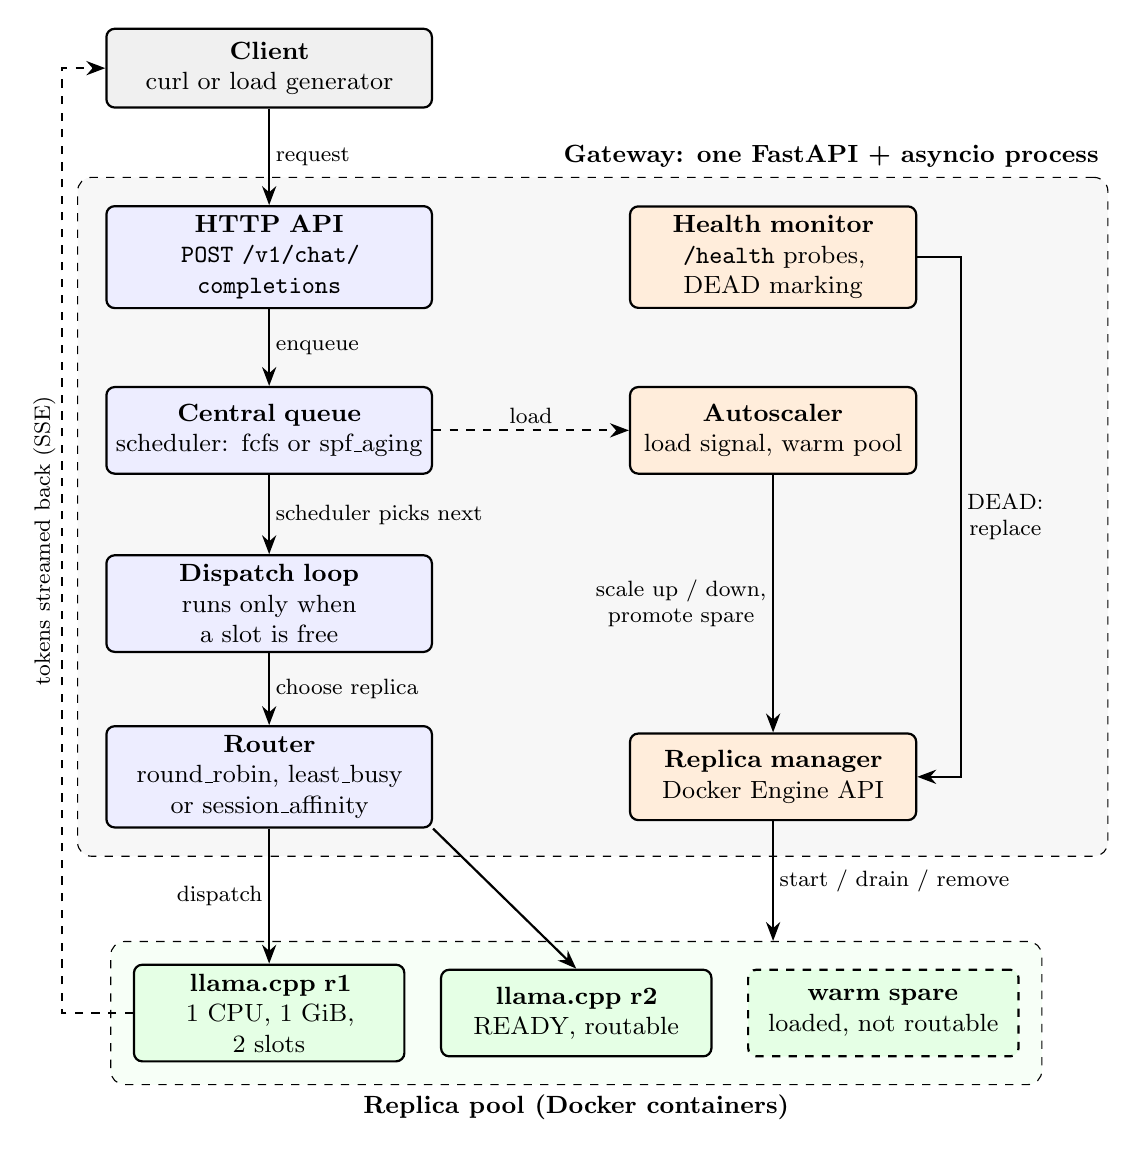
\begin{tikzpicture}[
  font=\small, >={Stealth[length=2.4mm]},
  data/.style={draw, thick, rounded corners=3pt, align=center, text width=3.9cm,
               minimum height=11mm, fill=blue!7},
  ctrl/.style={draw, thick, rounded corners=3pt, align=center, text width=3.4cm,
               minimum height=11mm, fill=orange!14},
  rep/.style={draw, thick, rounded corners=3pt, align=center, text width=3.2cm,
              minimum height=11mm, fill=green!10},
  ext/.style={draw, thick, rounded corners=3pt, align=center, text width=3.9cm,
              minimum height=10mm, fill=gray!12},
  arr/.style={->, thick},
  darr/.style={->, thick, dashed},
  lbl/.style={font=\footnotesize, inner sep=2pt, align=center}]
  % request path (left column, blue)
  \node[ext]  (client) at (0, 0)     {\textbf{Client}\\curl or load generator};
  \node[data] (api)    at (0,-2.4)   {\textbf{HTTP API}\\\code{POST /v1/chat/}\\\code{completions}};
  \node[data] (queue)  at (0,-4.6)   {\textbf{Central queue}\\scheduler: fcfs or spf\_aging};
  \node[data] (disp)   at (0,-6.8)   {\textbf{Dispatch loop}\\runs only when a slot is free};
  \node[data] (router) at (0,-9.0)   {\textbf{Router}\\round\_robin, least\_busy\\or session\_affinity};
  % control plane (right column, orange)
  \node[ctrl] (health) at (6.4,-2.4) {\textbf{Health monitor}\\\code{/health} probes, DEAD marking};
  \node[ctrl] (auto)   at (6.4,-4.6) {\textbf{Autoscaler}\\load signal, warm pool};
  \node[ctrl] (mgr)    at (6.4,-9.0) {\textbf{Replica manager}\\Docker Engine API};
  \coordinate (gwright) at (10.3,-2.4);   % room for the DEAD: replace label inside the box
  \begin{scope}[on background layer]
    \node[draw, dashed, rounded corners=5pt, fill=black!3, inner sep=10pt,
          fit=(api)(queue)(disp)(router)(health)(auto)(mgr)(gwright),
          label={[font=\small\bfseries, anchor=south east]north east:Gateway: one FastAPI + asyncio process}] (gw) {};
  \end{scope}
  % replica pool (bottom row, green)
  \node[rep]         (r1) at (0,-12.0)   {\textbf{llama.cpp r1}\\1~CPU, 1~GiB,\\2~slots};
  \node[rep]         (r2) at (3.9,-12.0) {\textbf{llama.cpp r2}\\READY, routable};
  \node[rep, dashed] (sp) at (7.8,-12.0) {\textbf{warm spare}\\loaded, not routable};
  \begin{scope}[on background layer]
    \node[draw, dashed, rounded corners=5pt, fill=green!3, inner sep=8pt, fit=(r1)(r2)(sp),
          label={[font=\small\bfseries]below:Replica pool (Docker containers)}] (pool) {};
  \end{scope}
  % request path
  \draw[arr] (client) -- node[lbl, right]{request} (api);
  \draw[arr] (api)    -- node[lbl, right]{enqueue} (queue);
  \draw[arr] (queue)  -- node[lbl, right]{scheduler picks next} (disp);
  \draw[arr] (disp)   -- node[lbl, right]{choose replica} (router);
  \draw[arr] (router) -- node[lbl, left]{dispatch} (r1);
  \draw[arr] (router.south east) -- (r2.north);
  \draw[darr] (r1.west) -- ++(-0.9,0) |- node[lbl, pos=0.25, sloped, above]{tokens streamed back (SSE)} (client.west);
  % control plane
  \draw[darr] (queue.east) -- node[lbl, above]{load} (auto.west);
  \draw[arr] (auto) -- node[lbl, left]{scale up / down,\\promote spare} (mgr);
  \draw[arr] (health.east) -- ++(0.55,0) |- node[lbl, pos=0.25, right]{DEAD:\\replace} (mgr.east);
  \draw[arr] (mgr) -- node[lbl, right, pos=0.5]{start / drain / remove} (pool.north -| mgr);
\end{tikzpicture}
\caption{Architecture. Left (blue): the request path. Requests wait only in the gateway's central
queue; the dispatch loop takes one only when some replica has a free slot, asks the router where it
goes and streams the replica's tokens back to the client. Right (orange): the control plane. The
health monitor, autoscaler and replica manager change the pool (green).}
\label{fig:arch}
\end{figure}

\begin{table}[!htbp]
\centering\small
\caption{Components.}
\label{tab:components}
\begin{tabularx}{\textwidth}{@{}P{3.0cm}P{5.0cm}L@{}}
\toprule
Component & File & Role \\
\midrule
Contracts & \code{gateway/interfaces.py} & Request, Replica, Config, EventLog, abstract components, registries \\
Gateway / dispatch & \code{gateway/main.py} & HTTP API, central queue, dispatch loop, streaming, retries, sessions, reload \\
Scheduler & \code{gateway/scheduler.py} & \code{fcfs}, \code{spf_aging} \\
Router & \code{gateway/router.py} & \code{round_robin}, \code{least_busy}, \code{session_affinity} \\
Replica manager & \code{gateway/replica_manager.py} & containers with \code{--cpus} / \code{--memory}, readiness, drain, removal \\
Health monitor & \code{gateway/health.py} & \code{/health} probes, DEAD marking, replacement \\
Autoscaler & \code{gateway/autoscaler.py} & load signal, scale up/down, warm pool \\
Logging & \code{gateway/logging_conf.py} & one line per event, tags SCHED / ROUTE / SCALE / HEALTH, monotonic \code{mono=} \\
Load generator & \code{loadgen/burst.py} & deterministic burst and session workloads \\
\bottomrule
\end{tabularx}
\end{table}

\paragraph{Key rule (decision 1).} Requests wait only in the gateway's queue and are dispatched only
to a free slot, so the scheduler alone decides who goes next and the router alone decides where.

\paragraph{Static versus dynamic infrastructure.} \code{docker-compose.yml} runs the static part,
the gateway itself, as one Compose service (image \code{gateway/Dockerfile}). Replicas are not
Compose services: the gateway creates, drains and removes them at run time through the Docker Engine
API~\cite{dockerapi,dockerpy}, because their number changes with load. The gateway container mounts the Docker socket (sibling
containers, not Docker-in-Docker), mounts the project at the same absolute path so \code{models_dir}
resolves to a host path the daemon can bind-mount, and uses host networking to reach replicas on the
\code{llmgw-net} bridge exactly as when it runs on the host. Verified with the real model
(\code{report/dry_runs/compose_check.log}): \code{docker compose up} started the gateway, which
started a replica and a warm spare and served a streamed request; \code{docker compose down} removed
every replica container.

% =====================================================================
\section{Mechanisms}
\label{sec:mech}

\subsection{Scheduling (Phase 3)}
\code{fcfs} serves in arrival order. \code{spf_aging} serves the request with the lowest
\[
  \text{priority} = \text{prompt\_tokens} - \alpha \cdot \text{wait\_s},
\]
with the prompt length estimated as characters / 4 and $\alpha$ = \code{aging_alpha}, i.e.\
shortest-job-first with aging~\cite{silberschatz}, with the prompt length as the job-size estimate. The aging
bound, stated precisely: a long request outranks every shorter request that arrives more than
$(p_\text{long} - p_\text{short}) / \alpha$ seconds after it; it still waits for those that arrived
before that point.

\subsection{Routing and session affinity (Phases 2 and 4)}
\code{round_robin} takes routable replicas in turn; \code{least_busy} picks the lowest
in-flight / slots. With a \code{session_id}, the gateway keeps the whole conversation (clients send
only the new message; a turn enters the history only when it completes) and \code{session_affinity}
keeps the session on one replica while that replica is routable (READY with a free slot); if it is
busy, draining or gone, the request falls back to \code{least_busy} and the session is re-mapped.
Requests without a \code{session_id} are routed \code{least_busy}. The history is replayed, so
answers never depend on one replica's cache.

\subsection{Fault tolerance (Phase 5)}
Probes run every \code{health_interval_s}; \code{health_fail_limit} failures, or a broken stream,
mark a replica DEAD. Its in-flight requests go back to the front of the queue (at most
\code{max_retries}; after that the client receives an error event), the container is removed and a
replacement started. On a retry the gateway compares the regenerated tokens with what the client
already has (greedy decoding, assumption 6), skips them and continues the stream; if they differ the
client gets an \code{llmgw_retry} event and the output restarts.

A replica whose container exits, or that never answers \code{/health}, while still loading is removed
(container and pool entry) and, if it was not a spare and the pool is below \code{min_replicas},
replaced (a failed spare is left to the warm-pool logic); after 3 consecutive load failures the
manager stops replacing them. That cap covers only the manager's own replacements: in
\code{warm_pool} mode the autoscaler starts a new spare whenever none exists, so with a persistently
bad image or model path spares would keep being started and removed, one at a time (no containers
accumulate; this path is not tested). A crash of a background task (dispatch loop, health monitor,
autoscaler) is logged at ERROR with its traceback.

\subsection{Autoscaling and warm pool (Phases 6--7)}
The load signal is (queued + in\_flight) / READY replicas, smoothed every 1 s. The autoscaler scales
up when the signal stays above \code{scale_up_threshold} for \code{scale_up_after_s} (promoting a warm
spare if there is one, else starting a container, at most one start at a time). It scales down when
the signal stays below \code{scale_down_threshold} for \code{scale_down_cooldown_s} and more than
\code{min_replicas} are READY, by draining the least-loaded READY replica (no new requests; in-flight
ones may finish for up to 30 s, then the container is stopped). With \code{prewarm: warm_pool},
\code{warm_pool_size} loaded-but-unroutable spares are kept (started under load or at idle). Spares
count toward \code{max_replicas} (our reading of decision 12; the frozen text does not say).

\subsection{Configuration reload and load generator (Phase 8)}
\code{POST /admin/reload} re-reads the configuration file, validates all of it first (invalid file:
HTTP 400, nothing changes), then applies it in one synchronous step; the scheduler and router are
rebuilt when their setting changed and queued requests (retries first) move to the new scheduler.
\code{loadgen/burst.py} sends deterministic workloads and records client-side timings.

\subsection{Cloud computing concepts demonstrated}
\label{sec:cloud}
The project realises, at single-host scale, the mechanisms that cloud platforms use to serve
variable load on shared infrastructure, for example the Kubernetes Horizontal Pod
Autoscaler~\cite{k8shpa} and warm pools in Amazon EC2 Auto Scaling~\cite{awswarm}
(Table~\ref{tab:cloud}). Everything runs on one machine;
multi-node orchestration (for example Kubernetes) is outside the scope of this project.

\begin{table}[!htbp]
\centering\small
\caption{Cloud computing concepts and where the project shows them.}
\label{tab:cloud}
\begin{tabularx}{\textwidth}{@{}P{3.4cm}LP{4.6cm}@{}}
\toprule
Concept & How the gateway realises it & Where it is shown \\
\midrule
Elastic horizontal scaling & replicas added and removed on a load signal, with hysteresis against flapping & Sec.~\ref{sec:prewarm}, \ref{sec:pools}; Fig.~\ref{fig:autoscale} \\
Resource isolation and quotas & each replica is a container with a cgroup CPU quota and memory limit (\code{--cpus}, \code{--memory}) & Sec.~\ref{sec:setup}; \code{replica_threads_real.txt} \\
Programmatic infrastructure & replicas created, drained and removed through the Docker Engine API; the static gateway service through Docker Compose & Sec.~\ref{sec:arch} \\
Health checking and self-healing & probes and broken streams mark replicas DEAD; requests are requeued and replicas replaced & Sec.~\ref{sec:single}; Fig.~\ref{fig:fault} \\
Cold starts and warm pools & loaded-but-unroutable spares trade idle cost for scale-up readiness & Sec.~\ref{sec:prewarm} \\
Load balancing and stateful placement & least-busy routing; session affinity to reuse a replica's prompt cache & Sec.~\ref{sec:affinity} \\
Graceful scale-in & draining: no new requests, in-flight work finishes before the container stops & Sec.~\ref{sec:prewarm} \\
Request scheduling on shared capacity & one central queue; fcfs vs shortest-prompt-first with aging & Sec.~\ref{sec:sched} \\
Observability & one structured, timestamped log line per decision; every figure is derived from these logs & Sec.~\ref{sec:setup} \\
\bottomrule
\end{tabularx}
\end{table}

% =====================================================================
\section{Experimental setup and methodology}
\label{sec:setup}

\paragraph{Machine and replicas.} Windows 11 laptop, WSL2 Ubuntu 24.04 (16 cores, 7.6 GiB visible),
Docker Engine 29.1.3. Qwen2.5-0.5B-Instruct Q4\_K\_M GGUF in \code{ghcr.io/ggml-org/}\allowbreak\code{llama.cpp:server};
each replica \code{--cpus 1 --memory 1g}, \code{-np} = slots, \code{-c} = slots $\times$ 2048,
\code{--cont-batching}. Configuration is \code{gateway/config.yaml}; each experiment changes only the
keys under comparison. The pre-warming and pool scripts print each condition's configuration and
check that only the compared keys differ; the scheduling and affinity scripts set the compared keys
explicitly.

\begin{table}[!htbp]
\centering\small
\caption{Workloads of the repeated experiments.}
\label{tab:workloads}
\begin{tabularx}{\textwidth}{@{}P{2.6cm}P{5.2cm}L@{}}
\toprule
Experiment & Script & Workload \\
\midrule
Pre-warming lifecycle (\ref{sec:prewarm}) & \code{scripts/demo3_prewarm.sh} & fresh gateway, 1 replica READY, 15 s idle, burst of 14 concurrent streamed clients (\code{max_tokens} 40), then idle until the pool is back at \code{min_replicas}; once with \code{prewarm: none}, once with \code{warm_pool} \\
Pool baseline (\ref{sec:pools}) & \code{scripts/compare_pools.sh} & the same burst after \code{min_replicas} are READY and 15 s idle; fixed1 (min = max = 1), fixed3 (min = max = 3), both \code{prewarm: none}; autoscale (\code{config.yaml} unchanged: min 1, max 3, warm pool) \\
Scheduling (\ref{sec:sched}) & \code{scripts/demo1_scheduling.sh} & 1 replica $\times$ 1 slot; A/B: a blocker, a long request L, 4 short requests 0.3 s apart (fcfs vs spf\_aging); C/D: a blocker, L, then a short request every 1 s, 16 in all (spf\_aging with $\alpha$ = 5 vs 0) \\
Session affinity (\ref{sec:affinity}) & \code{scripts/demo2_affinity.sh} & 2 replicas; 3 conversations $\times$ 5 turns sent strictly one after another with a \code{session_id}, \code{max_tokens} 12; session\_affinity vs round\_robin \\
\bottomrule
\end{tabularx}
\end{table}

\paragraph{Metrics.} All times come from the gateway log's monotonic \code{mono=} field.
\begin{itemize}
  \item \textbf{First token} (Sections~\ref{sec:prewarm}, \ref{sec:pools}): from the request's arrival
        in the gateway queue to its first token, so it includes queue wait.
  \item \textbf{Turn-2 TTFT} (Section~\ref{sec:affinity}): the gateway's \code{ttft_s}, measured from
        dispatch to the replica until the first token, so it excludes queue wait. In that sequential
        workload the queue is empty, so the difference is small, but the two metrics are not the
        same and are never compared with each other.
  \item \textbf{Makespan}: first arrival to last completion.
  \item \textbf{Wait} (Section~\ref{sec:sched}): time in the gateway queue, from arrival to selection by
        the scheduler (the scheduler's logged \code{wait_s}); it excludes service time.
  \item \textbf{load\_s}: time from just before \code{docker run} until the replica's \code{/health}
        returns 200; readiness is polled every 0.5 s, so load\_s and ``routable'' times have up to
        about 0.5 s resolution.
  \item \textbf{Container-seconds}: replica containers alive $\times$ time in the burst window, i.e.\
        CPU reserved (1 CPU each), not CPU used.
\end{itemize}

\paragraph{Repetition and aggregation.} The four experiments above were run 3 times each (12 runs,
2026-11-10, 19:59--20:38 UTC). The runs were sequential: each round ran the four scripts one after
another, so the rounds interleave the experiments and slow drift of the host affects all of them.
Each round used a fresh copy of the project without \code{report/evidence/}, so no committed evidence
could be overwritten, and before every script the runner checked that no replica container was left
and port 8000 was free (never violated). All 12 runs completed with 0 failed checks; none was
repeated or discarded. \code{report/aggregate_repeats.py} parses the 12 unedited output files
(\code{report/evidence/repeats/*_real_run<k>.txt}) and prints, per metric, the 3 per-run values,
their mean and their range (min--max) to \code{report/evidence/repeats/SUMMARY.txt}; the same parsed
values draw Figures~\ref{fig:prewarm}--\ref{fig:schedaff}. With $n = 3$, means and ranges are
descriptive; no significance test is used and none is claimed. Overlapping ranges are read as ``no
measurable difference in these runs''.

\paragraph{Real versus simulated.} Every demo was also run with a stand-in replica image (no model,
fixed 2 s ``load'', 20 tokens/s), labelled \code{SIMULATED} under \code{report/evidence/simulated/}.
Stand-in runs only check gateway behaviour; none of their numbers appear in this report.

% =====================================================================
\section{Default configuration and its justification}
\label{sec:defaults}

Defaults are those in \code{gateway/config.yaml}. They are reasonable engineering choices for this
machine and these workloads, not measured optima: no parameter was swept.

\begin{table}[!htbp]
\centering\footnotesize
\caption{Defaults, the evidence behind them, and the trade-off they make.}
\label{tab:defaults}
\begin{tabularx}{\textwidth}{@{}P{3.5cm}LL@{}}
\toprule
Default & Evidence & Trade-off and reason \\
\midrule
Autoscaling, \code{min_replicas 1}, \code{max_replicas 3}, \code{replica_cpus 1.0} &
Sec.~\ref{sec:pools}: autoscale's mean first-token latency (25.40 s) was close to fixed3 (25.91 s) and less than half of fixed1 (58.09 s); it held 2 containers while idle instead of 3. 3 $\times$ 1 CPU fits 16 cores (decision 12). &
Fixed capacity is ready before a burst and was faster to first token in 2 of 3 runs; autoscaling releases capacity when idle. With this burst, autoscaling gave comparable latency for less idle capacity. \\
\midrule
\code{scale_up_threshold 4.0}, \code{scale_up_after_s 5}, \code{scale_down_threshold 1.0}, \code{scale_down_cooldown_s 30} &
6 lifecycle runs (Sec.~\ref{sec:prewarm}) and the Phase 6 run: 1 $\rightarrow$ 3 replicas during the burst, drained back to 1 afterwards, no flapping. &
Separate thresholds and timers prevent oscillation at the cost of reacting about 5 s late to a burst and holding extra replicas after it (first released 22--30 s, back at \code{min_replicas} 53--61 s after the last request). \\
\midrule
\code{prewarm: warm_pool}, \code{warm_pool_size 1} &
Sec.~\ref{sec:prewarm}: the spare is routable at the trigger (0.00 s vs 1.29 s) and the new replica's first token came earlier (5.05 vs 7.72 s), but burst-level first-token latency and makespan did not differ measurably. &
Readiness against idle cost: one extra loaded container (1 CPU / 1 GiB reserved) at all times. Kept as the default because it removes load time from the scale-up path, which is expected to matter more when replica load is slow (larger models, uncached files; not measured here); on this host, with a 1.3--2.1 s cached load, \code{prewarm: none} is an equally defensible choice. \\
\midrule
\code{slots_per_replica 2} &
Phase 1 (single run): aggregate throughput 3.4 $\rightarrow$ 4.2 $\rightarrow$ 4.5 chunks/s at 1 / 2 / 3 concurrent requests; a third request waited 58 s for a slot. &
Small throughput gain from a second slot; more slots per 1-CPU replica add little, so capacity comes from more replicas. \\
\midrule
\code{scheduler: spf_aging}, \code{aging_alpha 5.0} &
Sec.~\ref{sec:sched}: short requests waited 8.65 s (spf\_aging) vs 13.11 s (fcfs), the long request 14.28 vs 6.31 s; under overload aging served L after 9 short requests instead of last (23.50 vs 39.83 s), identically in all 3 runs. &
Favours short prompts and bounds the long request's wait through aging; fcfs is fairer to arrival order. Not better in general: it trades long-request wait for short-request wait. \\
\midrule
\code{router: least_busy} &
Phase 2 (single run): least\_busy and round\_robin made identical choices when replicas filled evenly; no measured performance advantage. &
Behaviourally sound for unequal loads, and it is also what session\_affinity uses for requests without a \code{session_id}. \\
\midrule
\code{session_affinity} (not the default) &
Sec.~\ref{sec:affinity}: turn-2 TTFT 1.90 s vs 3.34 s with round robin for sequential conversations. &
Recommended when clients send \code{session_id}. Not the default because it was measured only with sequential conversations; its effect with many concurrent sessions was not measured. \\
\midrule
\code{health_interval_s 1.5}, \code{health_fail_limit 3}, \code{max_retries 2}, \code{default_temperature 0.0} &
Phase 5 (2 runs): killed replica detected in 0.46--0.66 s (broken stream), frozen replica in 7.55--7.77 s (probes); replacement READY 2.25--2.44 s after detection; all 8 retried requests completed on their first retry. &
Faster probing would detect frozen replicas sooner at more probe traffic. Greedy decoding makes prefix verification possible, but the final text of one prompt still differed from a fault-free run in 3 of 4 runs, so exact reproducibility is not guaranteed. \\
\bottomrule
\end{tabularx}
\end{table}

% =====================================================================
\section{Results (real model)}
\label{sec:results}

\subsection{Repeated measurements (3 runs each; mean, range in brackets)}
\label{sec:repeated}

\subsubsection{\texorpdfstring{Pre-warming over the full lifecycle: \code{prewarm: none} vs \code{warm_pool}}{Pre-warming over the full lifecycle: none vs warm pool}}
\label{sec:prewarm}

\begin{figure}[!htbp]
\centering
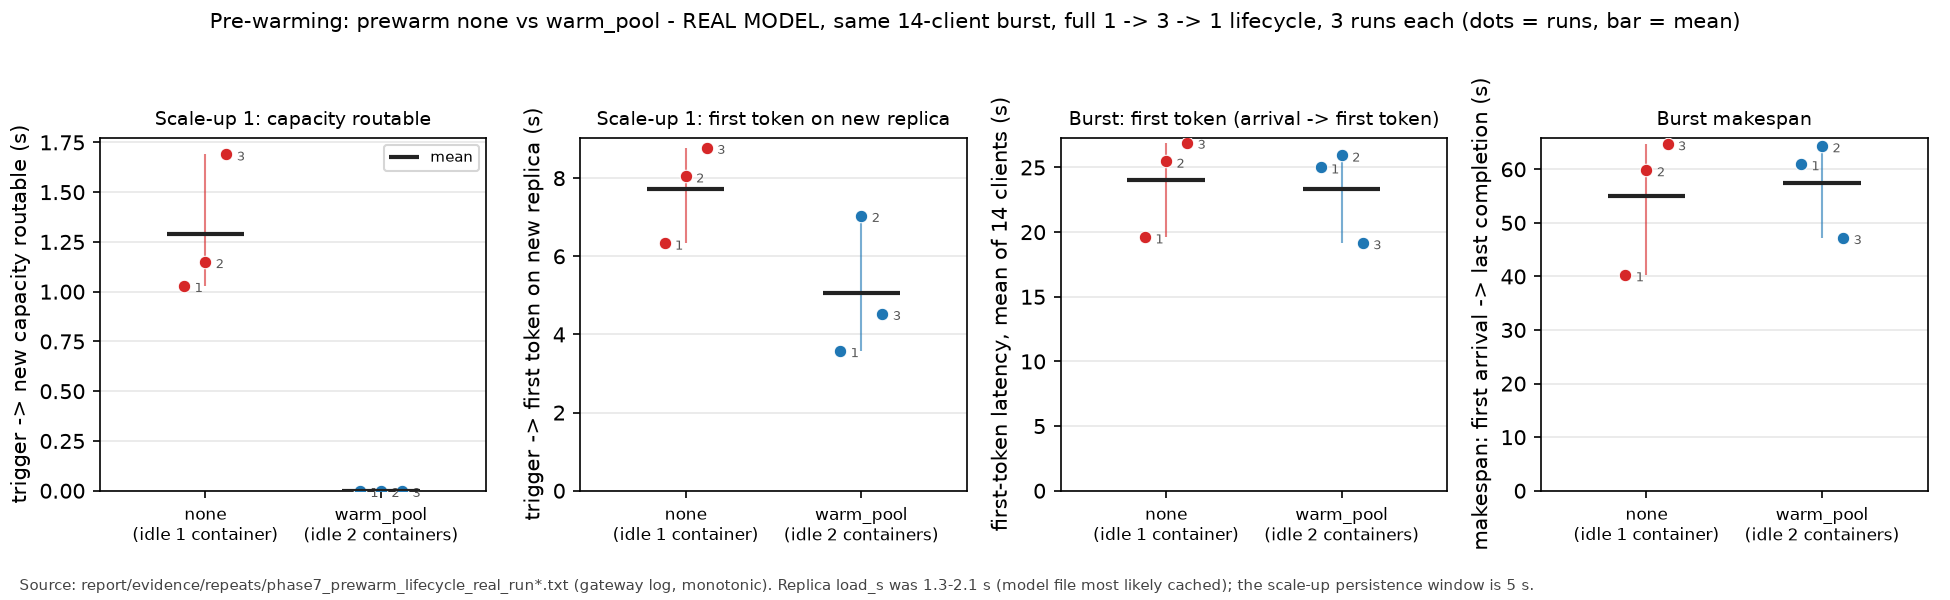
\includegraphics[width=\textwidth]{repeats_prewarm.png}
\caption{Pre-warming, 3 runs per mode. Dots are runs (numbered), bars are means.}
\label{fig:prewarm}
\end{figure}

\begin{table}[!htbp]
\centering\small
\caption{Pre-warming over the full lifecycle (3 runs per mode).}
\label{tab:prewarm}
\begin{tabularx}{\textwidth}{@{}LP{3.4cm}P{4.2cm}@{}}
\toprule
Metric & none & warm\_pool \\
\midrule
First scale-up: trigger $\rightarrow$ new capacity routable & 1.29 s \rng{1.03}{1.69} & 0.00 s in all runs \\
First scale-up: trigger $\rightarrow$ first token on the new replica & 7.72 s \rng{6.33}{8.78} & 5.05 s \rng{3.58}{7.04} \\
load\_s of that replica & 1.64 s \rng{1.33}{2.09} & 2.02 s \rng{1.98}{2.04}, loaded before it was needed \\
Burst: first-token latency, mean of 14 clients & 24.00 s \rng{19.61}{26.93} & 23.37 s \rng{19.16}{25.94} \\
Burst: completion latency, mean of 14 clients & 38.43 s \rng{29.89}{44.57} & 38.55 s \rng{31.04}{42.33} \\
Burst makespan & 54.95 s \rng{40.26}{64.71} & 57.51 s \rng{47.20}{64.34} \\
Last completion $\rightarrow$ back at \code{min_replicas} READY & 56.40 s \rng{53.97}{61.16} & 56.54 s \rng{52.87}{59.74} \\
Replica containers while idle & 1 & 2 (r1 + re-armed spare) \\
\bottomrule
\end{tabularx}
\end{table}

In all 6 runs the pool went 1 $\rightarrow$ 3 $\rightarrow$ 1 READY replicas: two scale-ups during
the burst, two drained scale-downs afterwards, no scale-up after the first scale-down, and in
\code{warm_pool} the spare was re-armed at the end. \textbf{The warm pool reduced replica start-up
delay on the scale-up path, but it did not show a robust end-to-end improvement for the burst.} The
new capacity was routable at the trigger instead of about 1.3 s later, and the new replica's first
token came earlier in each of the 3 pairs. The committed single Phase 7 run had the opposite sign for
that measure (none 6.87 s, warm\_pool 8.17 s), so over 4 runs warm\_pool was lower in 3. Burst-level
first-token latency, completion latency and makespan overlap almost completely. A replica loads in
1.3--2.1 s here, while the 5 s persistence window (\code{scale_up_after_s}) and queueing behind 2
slots per replica dominate what clients wait for; with cached model loads, decision 8's premise
(model load dominates scale-up delay) therefore does not hold on this host. The cost of the warm pool
is one additional loaded container held whenever the system is idle.

\subsubsection{Baseline: fixed pool of 1 vs fixed pool of 3 vs autoscaling}
\label{sec:pools}

\begin{itemize}
  \item A single replica (2 slots) gave about 2--2.8$\times$ the makespan and first-token latency of
        autoscaling in every run, and of fixed3 in runs 2 and 3; against the anomalous fixed3 run 1
        the ratios were 1.3$\times$ (makespan) and 1.7$\times$ (first token).
  \item \textbf{Fixed3 run 1 is anomalous}: every latency in that run was about 1.6$\times$ its runs
        2 and 3 values (makespan 98.18 s vs 58.50 / 60.06 s), although its routing (6/4/4 requests
        per replica) and replica load times (1.46--1.95 s) were normal. The demo scripts do not keep
        raw gateway logs, so the cause could not be identified; host interference is plausible but
        not shown. The run is kept in every mean and range.
  \item \textbf{Trade-off.} For this workload, autoscaling achieved first-token performance comparable
        to a permanently provisioned pool of 3 (means 25.40 vs 25.91 s), with fewer containers held
        idle (2 vs 3) and a lower observed mean makespan (59.84 vs 72.25 s). The makespan difference
        is driven by the fixed3 outlier: in runs 2 and 3 fixed3's makespan (58.50, 60.06 s) lay
        within autoscale's range, and its first-token mean (20.74, 22.17 s) was lower than
        autoscale's in every run, because its capacity exists before the burst. A burst arriving
        faster than the 5 s scale-up window, or a longer one, could change this balance.
\end{itemize}

\begin{figure}[!htbp]
\centering
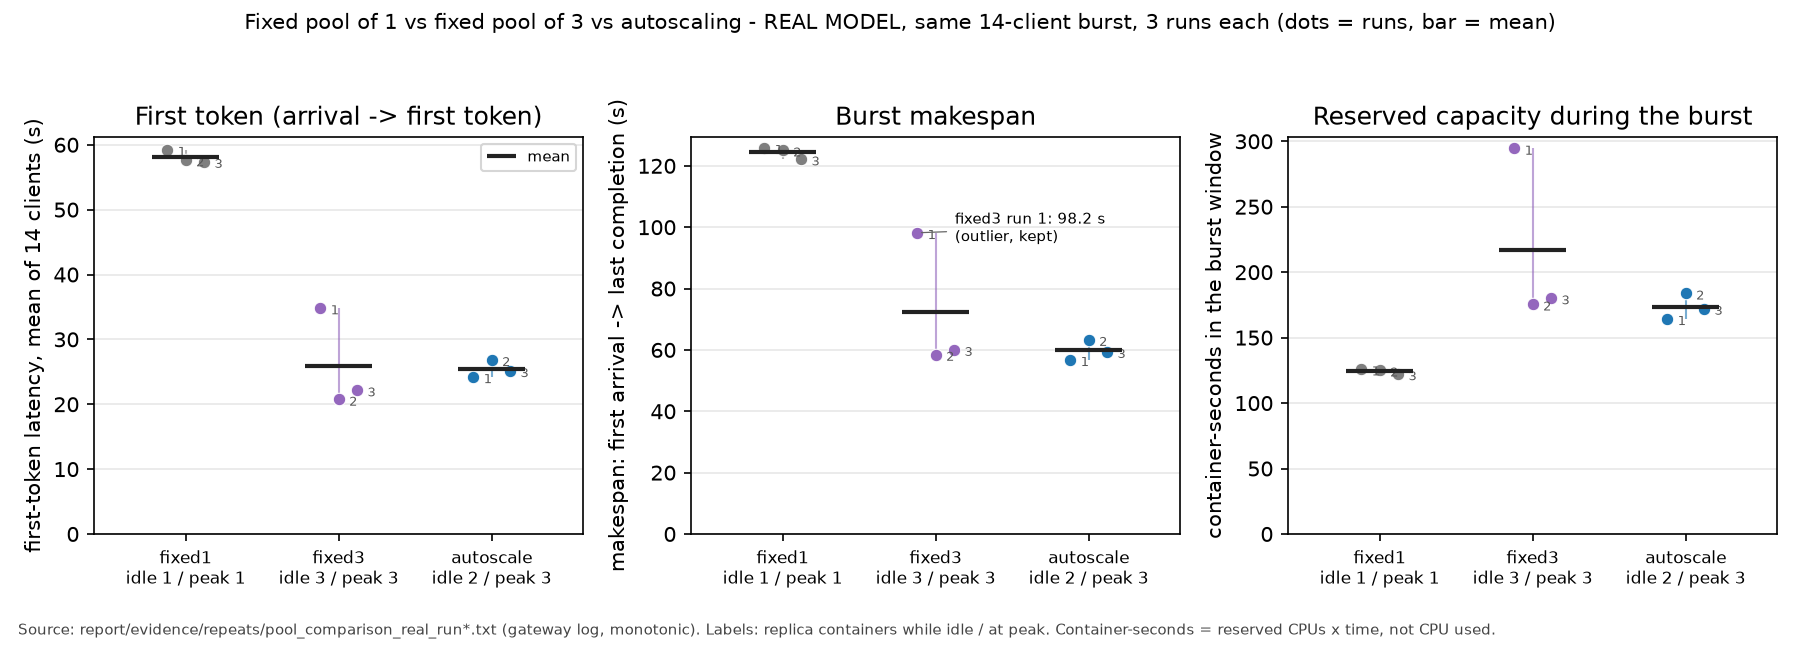
\includegraphics[width=\textwidth]{repeats_pool_comparison.png}
\caption{Same 14-client burst, 3 runs per pool. The fixed3 run 1 outlier is shown and included.}
\label{fig:pools}
\end{figure}

\begin{table}[!htbp]
\centering\small
\caption{Fixed pool of 1 vs fixed pool of 3 vs autoscaling (3 runs per pool).}
\label{tab:pools}
\begin{tabularx}{\textwidth}{@{}LP{3.1cm}P{3.1cm}P{3.1cm}@{}}
\toprule
Metric & fixed1 & fixed3 & autoscale \\
\midrule
First-token latency, mean of 14 clients & 58.09 s \rng{57.39}{59.24} & 25.91 s \rng{20.74}{34.83} & 25.40 s \rng{24.22}{26.85} \\
First-token latency, max & 110.21 s \rng{108.56}{111.97} & 54.03 s \rng{44.35}{72.45} & 44.89 s \rng{42.98}{47.23} \\
Completion latency, mean & 72.84 s \rng{71.74}{74.27} & 48.55 s \rng{38.25}{66.03} & 41.82 s \rng{38.69}{44.38} \\
Makespan & 124.38 s \rng{122.17}{125.88} & 72.25 s \rng{58.50}{98.18} & 59.84 s \rng{56.79}{63.35} \\
Replica containers while idle / at peak & 1 / 1 & 3 / 3 & 2 / 3 \\
Container-seconds in the burst window & 124.4 \rng{122.2}{125.9} & 216.7 \rng{175.5}{294.5} & 173.5 \rng{164.4}{183.9} \\
\bottomrule
\end{tabularx}
\end{table}

\subsubsection{Scheduling}
\label{sec:sched}

\begin{figure}[!htbp]
\centering
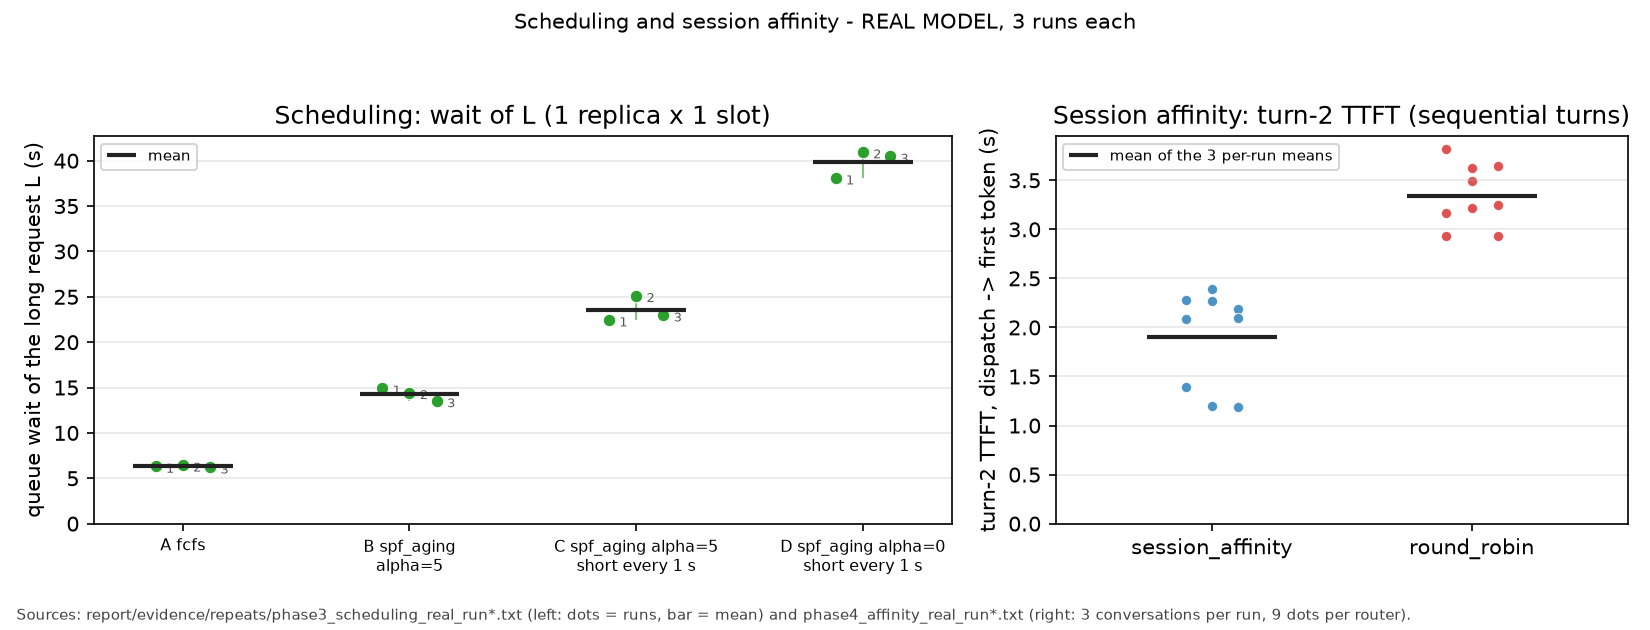
\includegraphics[width=\textwidth]{repeats_scheduling_affinity.png}
\caption{Left: wait of the long request L per scheduling run. Right: turn-2 TTFT, 9 conversations per router.}
\label{fig:schedaff}
\end{figure}

\begin{table}[!htbp]
\centering\small
\caption{Scheduling, 1 replica $\times$ 1 slot (3 runs per scenario).}
\label{tab:sched}
\begin{tabularx}{\textwidth}{@{}P{0.6cm}P{3.1cm}P{2.6cm}P{2.8cm}L@{}}
\toprule
Run & Policy & Wait of L & Mean wait of short requests & Service order \\
\midrule
A & fcfs & 6.31 s \rng{6.20}{6.43} & 13.11 s \rng{11.80}{14.16} & arrival order, all 3 runs \\
B & spf\_aging, $\alpha$ = 5 & 14.28 s \rng{13.51}{14.90} & 8.65 s \rng{8.25}{9.45} & all short requests before L, all 3 runs \\
C & spf\_aging, $\alpha$ = 5, overload & 23.50 s \rng{22.43}{25.12} & 14.72 s \rng{13.77}{16.52} & 9 short requests before L, 7 after, all 3 runs \\
D & spf\_aging, $\alpha$ = 0, overload & 39.83 s \rng{38.07}{40.95} & 13.68 s \rng{12.34}{14.37} & L last (after all 16), all 3 runs \\
\bottomrule
\end{tabularx}
\end{table}

The service order was identical in all 3 runs of every scenario, and so was the aging crossover in
C: the 9 short requests that arrived within the 9.2 s crossover bound ($(52 - 6)/5$) were served
before L and the 7 later ones after it; without aging (D) L was served last every time. Absolute
waits depend on host performance. Measured as the mean interval between consecutive scheduler
selections (the replica's time per request while the queue is non-empty), the replica was slower in
A, B and D than in the committed single Phase 3 run (2.61 / 1.96 / 2.06 s vs 1.70 / 1.55 / 1.31 s),
and L waited longer (6.31 / 14.28 / 39.83 s vs 5.25 / 10.22 / 27.28 s); D grows most because L waits
for all 16 short requests. In C the time per request was similar (2.16 vs 2.11 s) and so was L's wait
(23.50 vs 24.50 s). The gateway's decisions were the same; the ranking of L's wait
(A $<$ B $<$ C $<$ D) did not change.

\subsubsection{Session affinity (sequential conversations)}
\label{sec:affinity}

\begin{table}[!htbp]
\centering\small
\caption{Session affinity vs round robin, turn-2 TTFT (3 runs, per-run mean of 3 conversations).}
\label{tab:affinity}
\begin{tabular}{@{}lc@{}}
\toprule
 & Turn-2 TTFT \\
\midrule
session\_affinity & 1.90 s \rng{1.26}{2.22} \\
round\_robin & 3.34 s \rng{3.03}{3.56} \\
Difference (round\_robin $-$ affinity) & 1.44 s \rng{0.81}{2.18} \\
\bottomrule
\end{tabular}
\end{table}

All 9 turn-2 requests per router: affinity 1.19--2.39 s, round robin 2.93--3.82 s; the ranges do not
overlap (Figure~\ref{fig:schedaff}, right). In every run the affinity replica reused 44 prompt tokens
from its cache on turn 2 against 24--28 under round robin. The committed single Phase 4 run (1.553 vs
3.247 s) lies within these ranges. \textbf{This holds for the workload tested: one conversation at a
time, turns sent one after another, 2 replicas.} It does not show an advantage under concurrent
load, where pinning sessions can concentrate requests on one replica; that case was not measured.

\subsection{Single-run measurements}
\label{sec:single}

These were measured once (Phase 5: two runs) and are not repeated results.

\begin{figure}[!htbp]
\centering
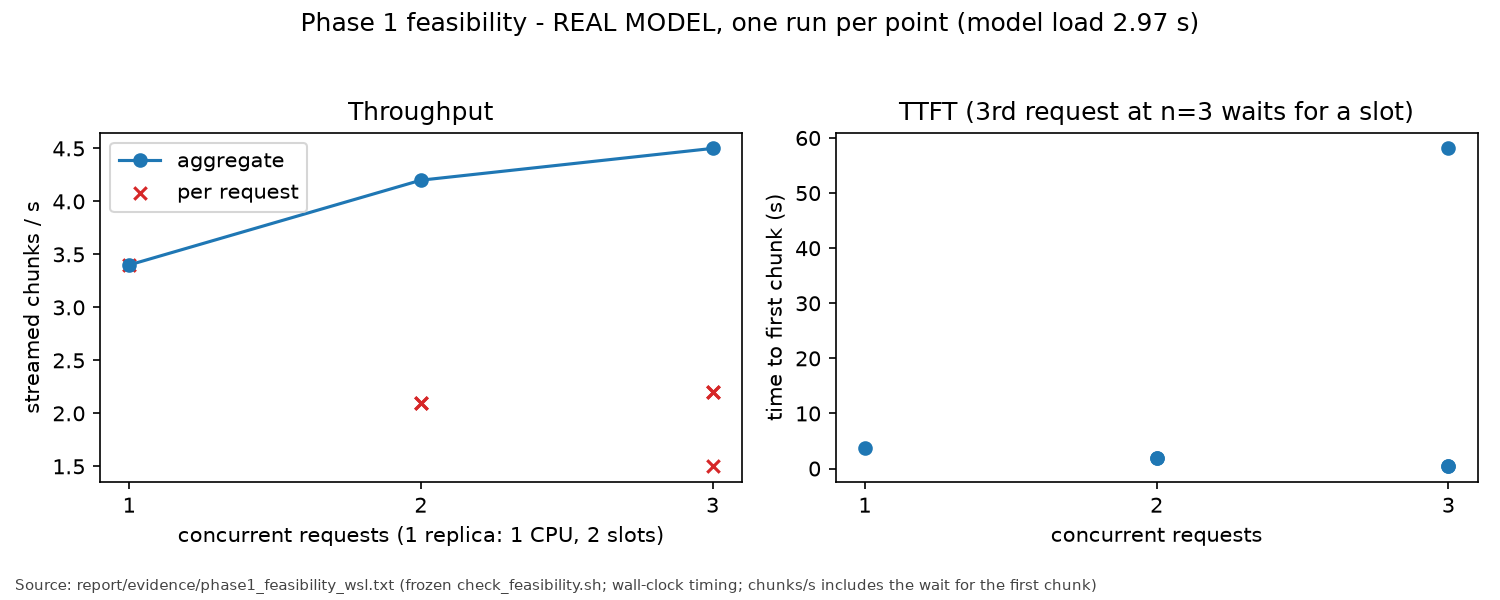
\includegraphics[width=0.92\textwidth]{phase1_feasibility.png}
\caption{One replica: model load 2.97 s; aggregate 3.4 / 4.2 / 4.5 chunks/s at 1 / 2 / 3 concurrent requests.}
\label{fig:feas}
\end{figure}

\begin{figure}[!htbp]
\centering
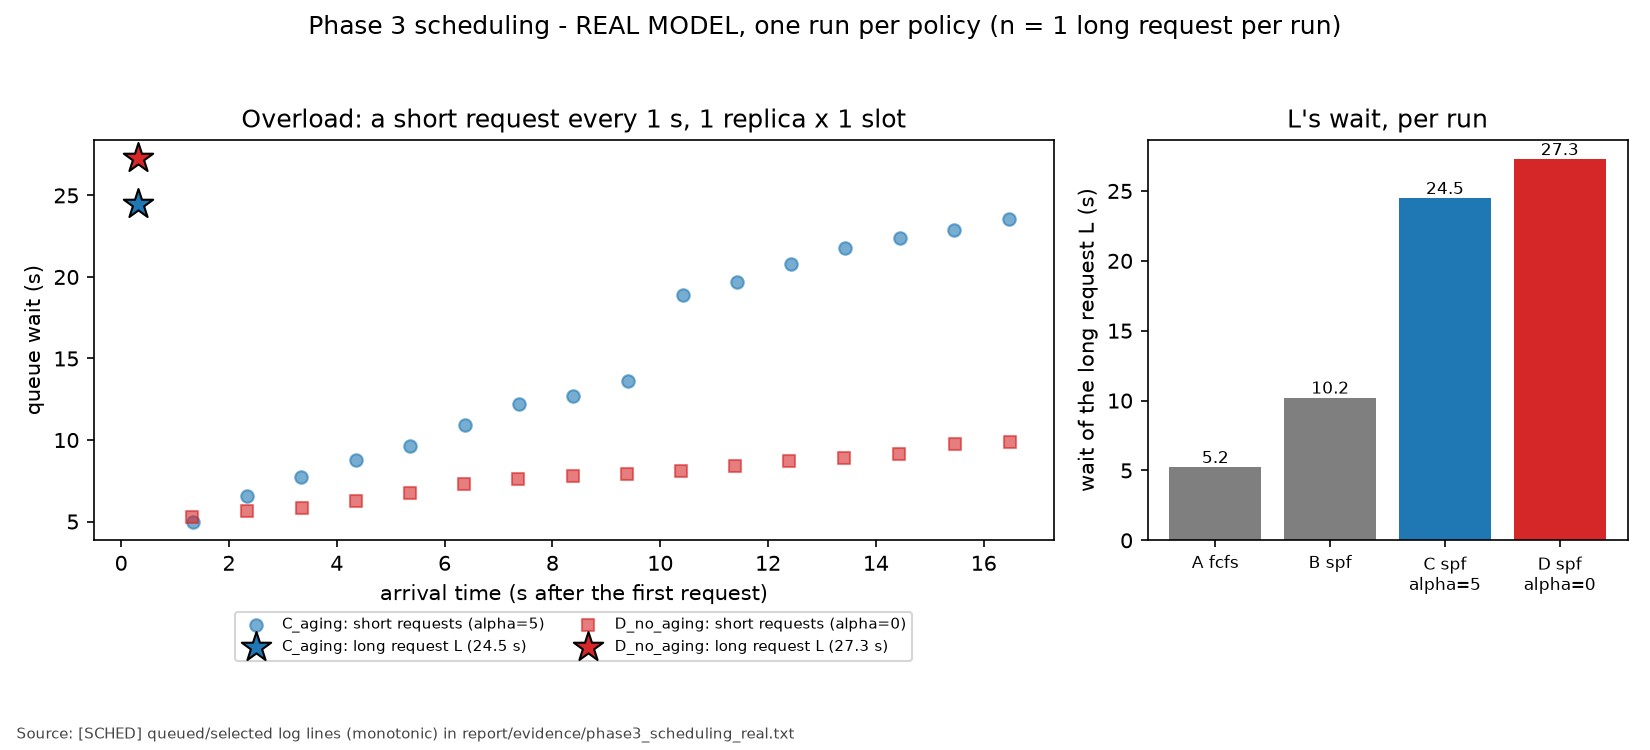
\includegraphics[width=0.92\textwidth]{phase3_scheduling.png}
\caption{Single Phase 3 run: queue wait of every request in the overload scenarios C and D, and L's wait in A--D.}
\label{fig:sched1}
\end{figure}

\begin{figure}[!htbp]
\centering
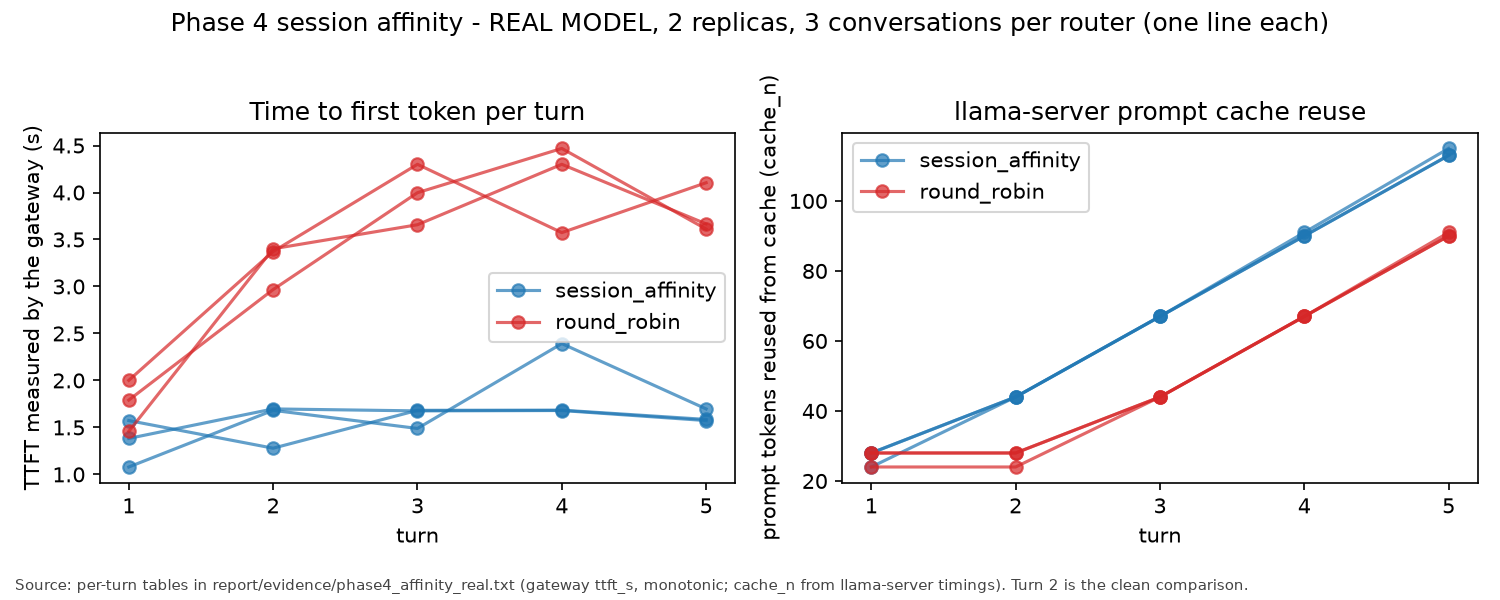
\includegraphics[width=0.92\textwidth]{phase4_affinity.png}
\caption{Single Phase 4 run: TTFT and prompt-cache reuse for all 5 turns of each conversation.}
\label{fig:aff1}
\end{figure}

\begin{figure}[!htbp]
\centering
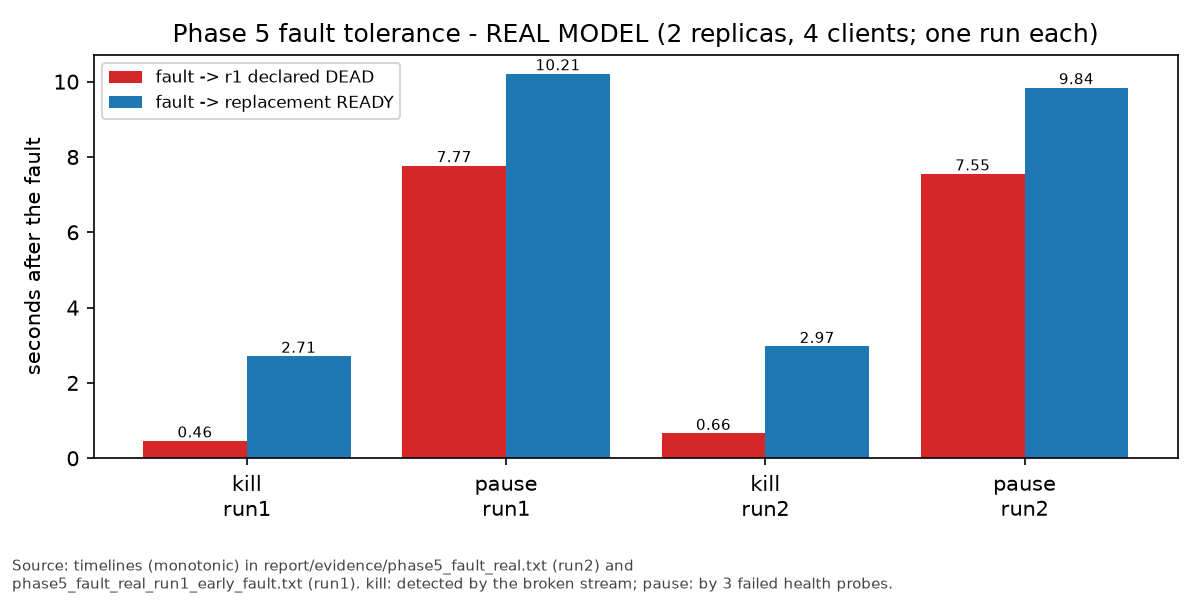
\includegraphics[width=0.8\textwidth]{phase5_fault.png}
\caption{Detection and replacement after \code{docker kill} / \code{docker pause}, two runs; all clients completed.}
\label{fig:fault}
\end{figure}

\begin{figure}[!htbp]
\centering
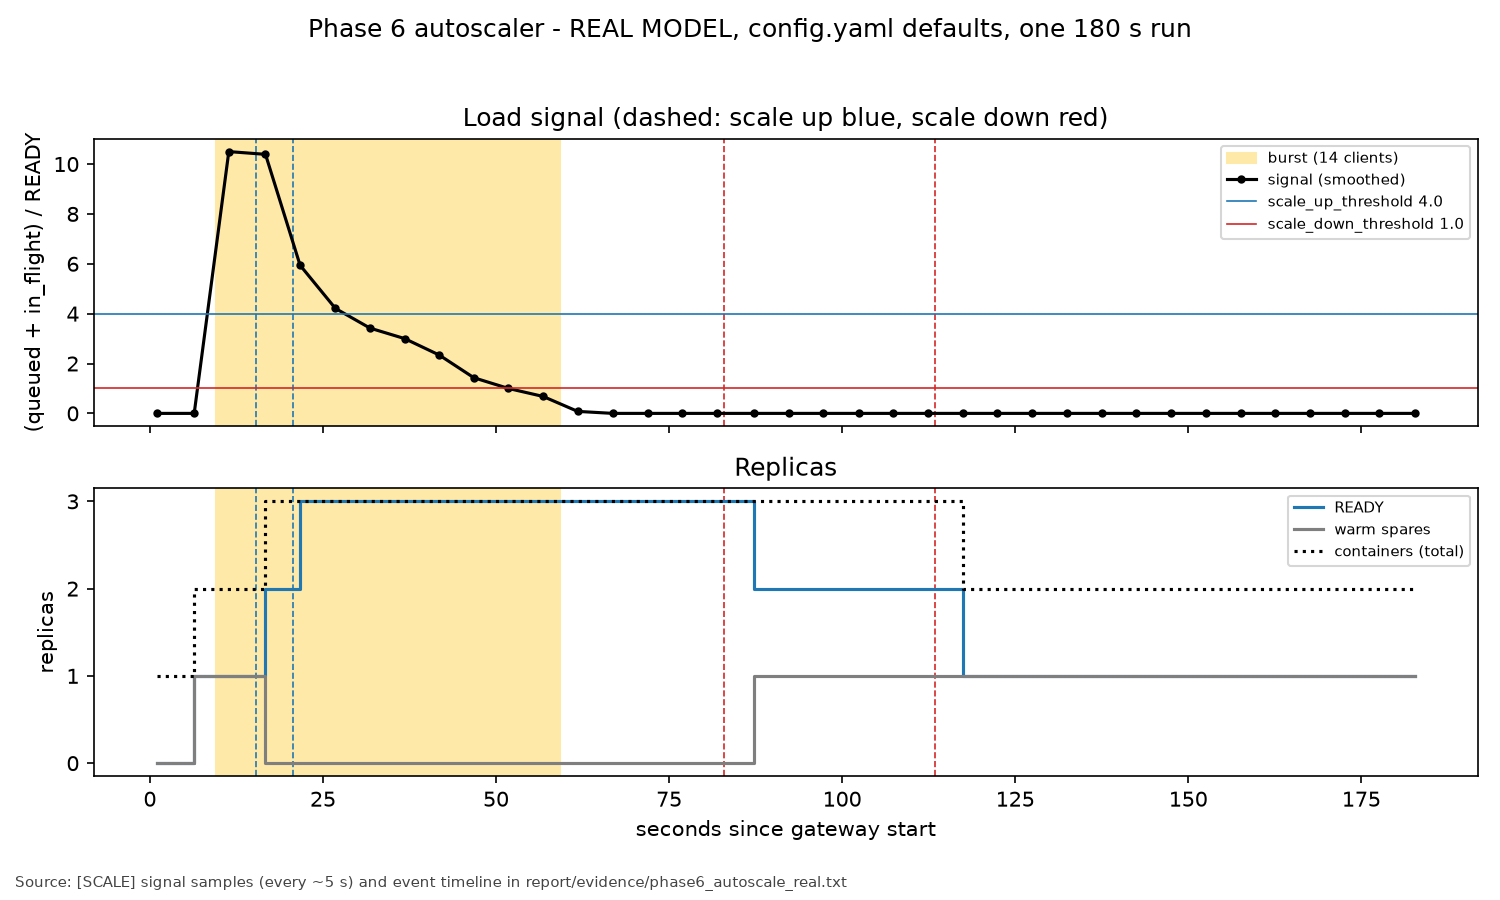
\includegraphics[width=0.92\textwidth]{phase6_autoscale.png}
\caption{Single 180 s run: scale up at 15.4 / 20.7 s, down at 82.9 / 113.4 s; no flapping.}
\label{fig:autoscale}
\end{figure}

\paragraph{Configuration switching (Phase 8, behaviour, real model).} In one gateway process, a
reload changed the service order (long request first under fcfs, last under spf\_aging), the
placement of a 4-turn session (r1 r2 r1 r2 $\rightarrow$ r1 r1 r1 r1) and the warm pool (none
$\rightarrow$ spare loaded in 1.94 s); an invalid file was rejected (HTTP 400) and the old settings
stayed in force. The single-run Phase 7 figure (\code{plots/phase7_prewarm.png}) is superseded by
Figure~\ref{fig:prewarm} and kept only with the Phase 9 record (\code{report/phase9_measurements.md}).

% =====================================================================
\section{Limitations and threats to validity}
\label{sec:limits}

\begin{itemize}
  \item \textbf{Small $n$.} 3 runs per condition for the repeated experiments; Phases 1, 5, 6 and 8
        are single runs (Phase 5: two). Requests inside a run are not independent repetitions. Means
        and ranges are descriptive; \textbf{no statistical significance is claimed}.
  \item \textbf{Uncontrolled host.} A Windows laptop running WSL2: background activity and power state
        were not controlled. Absolute times varied between sessions (Section~\ref{sec:sched}: up to
        about 1.6$\times$ longer per request than in the committed single run), and the 1-minute load
        average at script start ranged 0.02--5.15 (\code{run_log.txt}).
  \item \textbf{Order effects.} Within a round the order was always pre-warming $\rightarrow$ pools
        $\rightarrow$ scheduling $\rightarrow$ affinity, and within the pool comparison fixed1
        $\rightarrow$ fixed3 $\rightarrow$ autoscale.
  \item \textbf{Unexplained outlier.} Fixed3 run 1 (Section~\ref{sec:pools}) is about 1.6$\times$
        slower than its other runs; raw gateway logs were not retained by the demo scripts, so
        outliers can be described but not diagnosed. Earlier phases are likewise plotted from tables
        the scripts computed from their logs at run time.
  \item \textbf{One workload shape per question.} The scaling comparisons use one 14-client burst;
        the affinity result covers sequential conversations only; results may not transfer to other
        loads.
  \item \textbf{Cold model load was not measured.} The cold-load measurement was skipped (it needs
        \code{sudo} to drop the page cache, and in WSL2 that clears only the Linux VM's cache), and
        the unrun \code{cold_load_check.sh} script was removed. All load\_s values in this report
        were most likely measured with the model file already cached in memory, so they must not be
        read as verified cold-start times. This affects the interpretation of replica start-up (and
        therefore of the warm pool, whose benefit would grow with a slower load); it does not affect
        the scheduling, affinity or queueing measurements, which do not involve starting replicas.
  \item \textbf{Measurement details.} Phase 6 signal values are about 5 s samples; throughput
        (Phase 1) is counted in streamed chunks (about one token each) with the wall clock of the
        frozen feasibility script.
  \item \textbf{Thread count not matched to the CPU limit.} The replica command sets no \code{-t}; an
        inspection of one replica showed llama.cpp starting 8 threads under a 1-CPU quota
        (\code{report/evidence/replica_threads_real.txt}). Its effect on throughput and latency was
        not measured. All conditions used the same setting, so comparisons between them are like for
        like, but absolute per-replica numbers may differ from what a 1-thread setting would give.
  \item \textbf{Known implementation limits} (from reading the code; none occurred in the runs): the
        queue is unbounded, with no admission control (no 429/503); streams to replicas have no read
        timeout, so a replica that answers \code{/health} but stops generating would stall its
        clients; session histories are kept in memory without a bound and can outgrow the 2048-token
        context per slot, and concurrent turns of one session are not serialised; restarts of warm
        spares that fail while loading are not capped (Section~\ref{sec:mech}); configuration
        validation checks types, the allowed \code{prewarm} values and
        \code{min_replicas <= max_replicas} but not, for example, that the scale-down threshold is
        below the scale-up threshold.
  \item \textbf{Results apply only to this machine, model, image and these workloads.}
\end{itemize}

% =====================================================================
\section{Deviations from the frozen design}
\label{sec:deviations}

These are documented here; \code{ARCHITECTURE.md} itself was not edited.
\begin{itemize}
  \item Decision 4's aging bound is a crossover bound, not a bound on total wait (Phase 3 notes).
  \item Decision 7: draining waits for \code{in_flight == 0} for at most 30 s, then stops the
        container; a request still running then loses its stream and goes through the normal retry
        path (from the code; in every recorded scale-down the replica had drained,
        \code{drained=True}).
  \item Decision 8's premise (model load dominates scale-up delay) is not supported by the
        measurements (cached loads; a cold load was not measured).
  \item Decision 10: scheduler and router are rebuilt only when their setting changes (keeps affinity
        state).
  \item Decision 11: configuration reloads are logged with a fifth tag, \code{CONFIG}.
  \item Spares count toward \code{max_replicas}.
  \item Docker Compose covers only the static gateway service (\code{ARCHITECTURE.md} Section 1 lists
        the Compose plugin as ``only needed for the static part of the setup''); replicas stay under
        Engine API control.
  \item Additions outside the frozen layout: \code{tests/} (with the stand-in replica image),
        per-phase check scripts, \code{scripts/compare_pools.sh}, \code{report/aggregate_repeats.py},
        \code{docker-compose.yml} with \code{gateway/Dockerfile}, \code{requirements.txt},
        \code{LLMGW_CONFIG} / \code{LLMGW_LOG_FILE}, the \code{mono=} log field, the
        \code{session_id} request field, the \code{llmgw_retry} stream event, removal and bounded
        replacement of replicas that die while loading, and logging of crashed background tasks.
\end{itemize}

% =====================================================================
\section{Reproduction}
\label{sec:repro}

On a Linux host with Docker (here WSL2 Ubuntu), from the project root:

\noindent\begin{minipage}{\linewidth}   % keep the command block on one page
\begin{lstlisting}[language=bash]
python3 -m venv ~/llmgw-venv && source ~/llmgw-venv/bin/activate && pip install -r requirements.txt
bash scripts/check_feasibility.sh        # downloads the model, pulls the image, measures one replica
python -m pytest tests -v                # 107 tests (recorded: report/dry_runs/test_run.log)
uvicorn gateway.main:app --port 8000     # the gateway with gateway/config.yaml
docker compose up -d --build             # or: the gateway as a Compose service
bash scripts/run_all_demos.sh real       # every phase demo with the real model
bash scripts/run_all_demos.sh standin    # the same with the stand-in image (simulated)
bash scripts/compare_pools.sh real       # fixed1 / fixed3 / autoscale baseline (one run)
python report/measure.py                 # single-run plots from the committed evidence
python report/aggregate_repeats.py --plots > report/evidence/repeats/SUMMARY.txt
\end{lstlisting}
\end{minipage}

\code{run_all_demos.sh} runs the unchanged demo scripts in an isolated temporary copy of the
project, so committed evidence is never overwritten; \code{run_all_demos.sh real DIR} keeps that
run's outputs in \code{DIR}. A full real run took about 16 minutes on the submitted code (940 s,
Section~\ref{sec:dryruns}); the first two dry runs took about 14 minutes, before demo 3 was extended
to the full scale-down lifecycle. The repeated runs were made by running the four scripts of
Section~\ref{sec:setup} three times in this way.

% =====================================================================
\section{Final dry runs}
\label{sec:dryruns}

\code{scripts/run_all_demos.sh real} was run twice from a clean state on the demo machine (Phase 10),
before demo 3 was extended. Both runs passed all 8 demos (107 checks each, 0 failures, exit 0, about
14 minutes each), left no containers, processes or temporary files, and did not change any evidence
file. A third run on the submitted code (2026-11-11) passed all 8 demos with 115 checks (demo 3 now
has 21), 0 failures, in 940 s, with the same clean-up and evidence checks. The dry runs are
rehearsals: their outputs are discarded and are not used as measurements. Details, commands and the
console logs are in \code{report/dry_runs/DRY_RUNS.md}.

% =====================================================================
\section{Conclusion and future work}
\label{sec:conclusion}

We built a gateway that makes the queueing, placement, scaling and recovery decisions for
containerized LLM replicas explicit: one central queue, a scheduler that alone decides who goes
next, a router that alone decides where, and a replica manager, health monitor and autoscaler that
change the pool through the Docker Engine API, with every policy switchable at run time and every
decision logged. On this machine, with this model and these workloads, the measurements support
the following conclusions.

\begin{itemize}
  \item \textbf{Elastic capacity pays off for bursts.} Autoscaling gave first-token latency
        comparable to a permanently provisioned pool of three (25.40 vs 25.91 s mean) while holding
        2 containers idle instead of 3, and less than half that of a single replica (58.09 s).
        Fixed capacity still reached the first token sooner in 2 of 3 runs, because it exists
        before the burst.
  \item \textbf{Scheduling is a trade-off, not a free gain.} Shortest-prompt-first cut the short
        requests' mean wait from 13.11 to 8.65 s and raised the long request's from 6.31 to
        14.28 s; aging bounded its starvation (served after 9 short requests instead of last,
        23.50 vs 39.83 s), with the same service order in every run.
  \item \textbf{Placement matters for stateful work.} Session affinity lowered turn-2 time to first
        token from 3.34 to 1.90 s for sequential conversations, with more prompt-cache reuse (44 vs
        24--28 tokens).
  \item \textbf{Failures are handled inside the gateway.} A killed replica was detected in
        0.46--0.66 s and a frozen one in 7.55--7.77 s; replacements were READY 2.25--2.44 s after
        detection, and all 8 retried requests completed on their first retry (Phase 5, two runs).
  \item \textbf{A warm pool helps only when start-up is the bottleneck.} The spare made new
        capacity routable at once, but with cached model loads of 1.3--2.1 s the 5 s scale-up
        window and queueing dominated what clients waited for, so burst-level latency did not
        improve measurably.
\end{itemize}

The broader lesson for this host is that the scale-up delay clients saw was set mainly by the
autoscaler's own persistence window and by queueing, not by starting a replica.

\paragraph{Future work.} Each item follows from a limitation in Section~\ref{sec:limits}.
\begin{itemize}
  \item \textbf{Cold starts:} measure model loads with the page cache dropped (on a native Linux
        host) and with larger models, to test whether the warm pool's benefit grows with load time,
        as decision 8 assumed.
  \item \textbf{Thread count:} set llama.cpp's \code{-t} to match the 1-CPU quota and measure its
        effect on per-replica throughput.
  \item \textbf{Robustness:} admission control (a bounded queue answering 429/503), a read timeout
        on replica streams, session histories bounded to the context window, serialised turns
        within a session, and a cap on warm-spare restarts.
  \item \textbf{Wider experiments:} more runs per condition, other burst shapes, a sweep of
        \code{scale_up_after_s} and the thresholds (none was swept), session affinity with many
        concurrent sessions, and demo scripts that keep raw gateway logs so outliers such as fixed3
        run 1 can be diagnosed.
  \item \textbf{Multiple machines:} move replica management from the Docker Engine API to an
        orchestrator such as Kubernetes~\cite{k8shpa} and compare the gateway's own scaling policy
        with its Horizontal Pod Autoscaler; larger models would call for a GPU serving engine such
        as vLLM~\cite{vllm} behind the same gateway.
\end{itemize}

% =====================================================================
\begin{thebibliography}{10}
\addcontentsline{toc}{section}{References}
\small
\bibitem{qwen25} Qwen Team (A.~Yang et al.), ``Qwen2.5 Technical Report,'' arXiv:2412.15115, 2024.
\bibitem{qwengguf} Qwen, ``Qwen2.5-0.5B-Instruct-GGUF'' (model files), Hugging Face,
  \url{https://huggingface.co/Qwen/Qwen2.5-0.5B-Instruct-GGUF}.
\bibitem{llamacpp} ggml-org, ``llama.cpp: LLM inference in C/C++,''
  \url{https://github.com/ggml-org/llama.cpp}.
\bibitem{fastapi} S.~Ramírez, ``FastAPI,'' \url{https://fastapi.tiangolo.com/}.
\bibitem{dockerapi} Docker Inc., ``Docker Engine API,'' \url{https://docs.docker.com/reference/api/engine/}.
\bibitem{dockerpy} Docker Inc., ``Docker SDK for Python,'' \url{https://docker-py.readthedocs.io/}.
\bibitem{silberschatz} A.~Silberschatz, P.~B. Galvin and G.~Gagne, \emph{Operating System
  Concepts}, 10th ed., Wiley, 2018 (CPU scheduling: shortest-job-first and aging).
\bibitem{k8shpa} The Kubernetes Authors, ``Horizontal Pod Autoscaling,''
  \url{https://kubernetes.io/docs/tasks/run-application/horizontal-pod-autoscale/}.
\bibitem{awswarm} Amazon Web Services, ``Decrease latency for applications with long boot times
  using warm pools,'' Amazon EC2 Auto Scaling User Guide,
  \url{https://docs.aws.amazon.com/autoscaling/ec2/userguide/ec2-auto-scaling-warm-pools.html}.
\bibitem{vllm} W.~Kwon et al., ``Efficient Memory Management for Large Language Model Serving with
  PagedAttention,'' in \emph{Proc.\ 29th ACM Symposium on Operating Systems Principles (SOSP)}, 2023.
\end{thebibliography}
\noindent{\small Web pages were accessed in November 2026.}

% =====================================================================
\clearpage
\appendix
\section{Evidence and artefacts}
\label{app:evidence}

\begin{table}[!htbp]
\centering\small
\caption{Where the evidence behind this report is kept (all paths relative to the project root).}
\label{tab:evidence}
\begin{tabularx}{\textwidth}{@{}P{7.6cm}L@{}}
\toprule
Path & Contents \\
\midrule
\code{report/evidence/*_real.txt} & single-run real-model evidence of Phases 1--8 (unedited demo output) \\
\code{report/evidence/repeats/} & the 12 repeated real-model runs, \code{run_log.txt}, \code{SUMMARY.txt}, \code{NOTES.md} \\
\code{report/evidence/replica_threads_real.txt} & llama.cpp thread-count inspection of one replica \\
\code{report/evidence/simulated/} & stand-in (simulated) runs; behaviour checks only, not used for numbers \\
\code{report/plots/} & all figures, regenerated from the evidence by \code{measure.py} and \code{aggregate_repeats.py} \\
\code{report/dry_runs/} & dry-run console logs and state checks, the recorded test run and the Compose check \\
\code{report/phase9_measurements.md} & the Phase 9 single-run measurement record \\
\code{ARCHITECTURE.md} & the frozen design, decisions and ten-phase plan \\
\bottomrule
\end{tabularx}
\end{table}

\end{document}
